\chapter{\IfLanguageName{dutch}{Stand van zaken}{State of the art}}%
\label{ch:stand-van-zaken}

% Tip: Begin elk hoofdstuk met een paragraaf inleiding die beschrijft hoe
% dit hoofdstuk past binnen het geheel van de bachelorproef. Geef in het
% bijzonder aan wat de link is met het vorige en volgende hoofdstuk.

% Pas na deze inleidende paragraaf komt de eerste sectiehoofding.

Dit hoofdstuk bespreekt de huidige kennis en ontwikkelingen met betrekking tot databases in Edge Computing-omgevingen en relevante data-partitioneringstechnieken.
De literatuurstudie focust op de essentie van Edge Computing,
 de functie van databases in deze omgevingen en de specifieke technieken voor partitionering die kunnen helpen bij het verbeteren van de prestaties.
 Dit overzicht biedt de benodigde achtergrondinformatie om de resultaten van het praktische deel van dit onderzoek beter te kunnen interpreteren en in een context te plaatsen.

\section{Definitie van Kernbegrippen}

In dit onderzoek worden verschillende technische termen gebruikt. Hieronder volgt een overzicht van de kernbegrippen die essentieel zijn voor het begrijpen van de literatuurstudie en de daaropvolgende analyse:
 
\begin{itemize}
    \item \textbf{Sharding:} Dit is een techniek waarbij een database wordt opgesplitst in kleinere, beter beheersbare delen die afzonderlijk op verschillende servers worden opgeslagen. Elk deel, of shard, bevat een subset van de gegevens en helpt de schaalbaarheid en prestaties te verbeteren \autocite{Mahmud2020}.

    \item \textbf{Eventual Consistency:} Een consistentiemodel waarbij gegevens in een gedistribueerd systeem na verloop van tijd consistent worden. Dit model wordt vaak toegepast in systemen waar lage latentie belangrijker is dan directe consistentie zoals in IoT-omgevingen \autocite{Cao2020}.

    \item \textbf{Cyclisch (Round-robin):} Bij round-robin partitionering worden records gelijkmatig verdeeld over de beschikbare partities in een herhalend (cyclisch) patroon. Dit betekent dat de data in volgorde over de partities wordt verdeeld en wanneer de laatste partitie bereikt is, wordt het proces opnieuw gestart bij de eerste partitie. Dit zorgt voor een gelijkmatige belasting, maar kan inefficiënt zijn voor gerelateerde queries, omdat de data over verschillende partities is verspreid \autocite{Ponnusamy2024}.

    \item \textbf{Hypertables:} Dit is een concept dat wordt gebruikt in TimescaleDB voor het efficiënt beheren van tijdgebaseerde gegevens. Hypertables zijn eigenlijk tabellen die automatisch worden verdeeld op basis van tijdsintervallen, waardoor gegevens snel kunnen worden opgeslagen en opgehaald. Dit maakt ze uitermate geschikt voor toepassingen die veel tijdsgebonden gegevens genereren zoals IoT-sensoren \autocite{TimescaleDBDocumentation}.

    \item \textbf{ACID-transacties:} ACID staat voor \textit{Atomicity}, \textit{Consistency}, \textit{Isolation} en \textit{Durability}. Deze vier eigenschappen zorgen ervoor dat een database altijd in een consistente en betrouwbare staat blijft, zelfs bij fouten. Dit betekent dat elke bewerking in de database als een ononderbroken geheel wordt uitgevoerd (atomiciteit), gegevens op een consistente manier worden opgeslagen (consistentie), gelijktijdige bewerkingen van verschillende gebruikers geen conflicten veroorzaken (isolatie) en eenmaal opgeslagen gegevens niet verloren gaan (duurzaamheid). Dit is essentieel voor systemen die met kritieke gegevens werken \autocite{Cao2020}.

    \item \textbf{MVCC (Multi-Version Concurrency Control):} Dit is een techniek die ervoor zorgt dat meerdere gebruikers gelijktijdig gegevens kunnen bewerken zonder elkaar in de weg te zitten. MVCC maakt gebruik van meerdere versies van gegevens, zodat lezers altijd de meest recente versie kunnen zien zonder te wachten op schrijfbewerkingen en schrijvers kunnen hun wijzigingen doorvoeren zonder andere gebruikers te blokkeren. Dit maakt het systeem efficiënter en zorgt voor een betere gelijktijdige toegang tot gegevens \autocite{Wiseso2020PerformanceAnalysis}.

    \item \textbf{Query-optimalisaties:} Dit zijn technieken die worden gebruikt om zoekopdrachten in een database sneller en efficiënter te maken. Bijvoorbeeld door de manier waarop gegevens worden opgehaald te verbeteren of door de database zo in te richten dat zoekopdrachten minder tijd kosten. Dit is belangrijk in systemen waar snel toegang tot grote hoeveelheden data vereist is zoals bij real-time toepassingen \autocite{Gyorodi2015comparative}.
\end{itemize}

\section{Edge Computing: Definitie en Belang}

Edge Computing is een gedistribueerde IT-architectuur die clientgegevens aan de rand van het netwerk verwerkt in plaats van afhankelijk te zijn van een centrale locatie voor gegevensverwerking \autocite{Shi2018}.
 Het boek van Weisong Shi, Quan Zhang en Jie Cao behandelt de basis van edge computing en benadrukt de voordelen van deze architectuur met betrekking tot betrouwbaarheid, latentie en bandbreedte.

De toenemende hoeveelheid Internet of Things (IoT) apparaten die aanzienlijke datastromen genereren, speelt een belangrijke rol bij het aanmoedigen van Edge Computing \autocite{Shi2016}.
 Door rekenkracht en opslagcapaciteit dichter bij de bron te brengen, kan edge computing de prestaties en efficiëntie van dataverwerking aanzienlijk verbeteren, wat volgens Shi een oplossing biedt voor de uitdagingen waarmee cloud computing te maken heeft.

Taheri en Deng wijzen erop dat edge computing een oplossing biedt voor de beperkingen van cloud computing, met betrekking tot bandbreedte en latentie \autocite{Taheri2020}.
 Lage latentie verwijst naar de minimale vertraging tussen het uitvoeren van een bewerking zoals een gegevensopvraag en het ontvangen van een resultaat. In Edge Computing is lage latentie essentieel omdat data vaak lokaal wordt verwerkt op randapparaten in plaats van via een centraal datacenter, wat de responstijd aanzienlijk verkort \autocite{Taheri2020}. Dit is met name belangrijk voor toepassingen zoals realtime monitoring of IoT-apparaten, waar vertragingen directe impact kunnen hebben op prestaties of beslissingen.

Betrouwbare gegevensconsistentie betekent dat gegevens overal in het gedistribueerde systeem uniform blijven, zelfs bij gelijktijdige bewerkingen of beperkte netwerkconnectiviteit. Edge-databases zoals ObjectBox gebruiken mechanismen zoals transactionele consistentie en synchronisatieprotocollen om ervoor te zorgen dat gegevens tussen lokale apparaten en de cloud consistent blijven \autocite{Rahmani2018, Taheri2020}. Dit maakt ze ideaal voor situaties waarin netwerkverbindingen tijdelijk kunnen wegvallen, maar de betrouwbaarheid van de gegevens absoluut essentieel is.

Taheri en Deng benadrukken dat deze databases specifiek zijn geoptimaliseerd om te functioneren in omstandigheden met beperkte netwerkconnectiviteit, wat ze bijzonder geschikt maakt voor Edge Computing-omgevingen waar de netwerkbandbreedte en stabiliteit kunnen variëren \autocite{Taheri2020}.
 Door de verwerking en opslag naar de rand van het netwerk te verplaatsen, kunnen aanzienlijke verbeteringen in prestaties en efficiëntie worden bereikt, wat essentieel is voor toepassingen die een snelle en betrouwbare gegevensverwerking vereisen.

\section{Database on Edge}
De verschuiving naar gedecentraliseerde Edge Computing is onmiskenbaar en wordt steeds belangrijker door de enorme hoeveelheid data die dagelijks gegenereerd wordt door de toenemende hoeveelheid verbonden apparaten.
 Deze data-explosie benadrukt het belang van Edge Computing, dat volgens de Gartner Hype Cycle zijn hoogtepunt bereikt.

\begin{figure}[h]
    \centering
    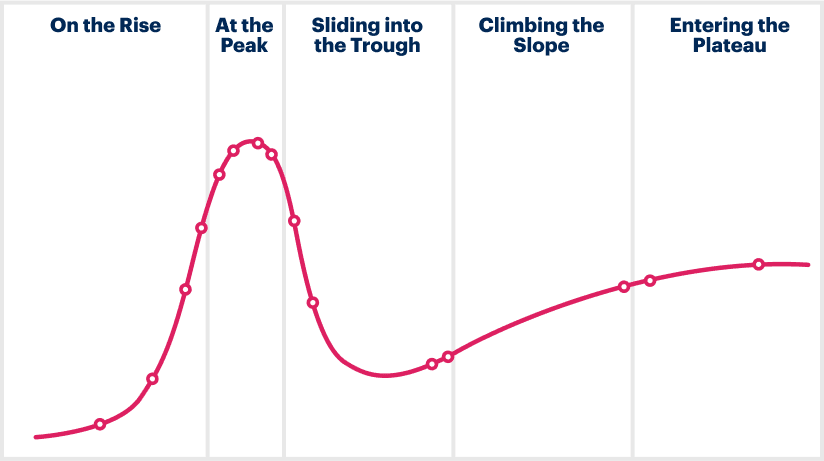
\includegraphics[width=0.5\textwidth]{hype-cycle-illustation.png}
    \caption{Gartner Hype Cycle, bron: \autocite{Gartner2023}}
    \label{fig:hype-cycle}
\end{figure}
 
De Gartner Hype Cycle laat zien hoe nieuwe technologieën aanvankelijk populair worden en geaccepteerd raken, maar vaak na een periode van teleurstelling pas echt volwassen worden en hun potentieel bereiken.

Edge Computing draait niet alleen om hardware, het gaat ook om hoe systemen aan de rand van het netwerk werken, waarbij gedistribueerde systemen worden ingezet in plaats van centrale organisatie. Door de verwerking en opslag naar de rand van het netwerk te verplaatsen, biedt Edge Computing oplossingen voor uitdagingen zoals latentie en afhankelijkheid van netwerkconnectiviteit, die in centrale cloudsystemen vaak een belemmering vormen. Dit maakt het mogelijk om bijna in realtime te reageren en zonder internetverbinding te functioneren, wat de kosten verlaagt voor dataoverdracht naar centrale servers.

Edge Databases spelen een cruciale rol in deze gedistribueerde omgeving. Ze zorgen ervoor dat gegevens efficiënt worden opgeslagen en gedeeld tussen verschillende apparaten in een verspreide omgeving, waarbij ze perfect aansluiten op moderne technologiestacks.

In tegenstelling tot klassieke databases, die vaak zijn ontworpen voor centrale dataopslag en verwerking in datacenters of op cloudservers, brengen edge-databases de gegevensverwerking dichter bij de bron zoals IoT-apparaten of sensoren.
 Klassieke databases vertrouwen sterk op continue netwerkverbindingen om toegang te bieden tot data die op centrale servers worden opgeslagen, wat latentie en afhankelijkheid van bandbreedte kan verhogen.
Dit maakt ze minder geschikt voor toepassingen waarbij real-time gegevensverwerking of directe toegang essentieel zijn.

Edge-databases daarentegen zijn ontworpen met specifieke optimalisaties voor lokale verwerking en tijdelijke opslag, zelfs bij beperkte of intermitterende netwerkverbindingen. Ze bieden voordelen zoals:
\begin{itemize}
    \item \textbf{Lagere latentie:}  
    In tegenstelling tot centrale databases, waarbij data-overdracht naar een externe server noodzakelijk is, worden gegevens in edge-databases lokaal verwerkt. Dit leidt tot aanzienlijk kortere responstijden, wat cruciaal is voor realtime toepassingen zoals IoT-apparaten of monitoring. Taheri en Deng benadrukken dat lokale verwerking latency vermindert, waardoor gebruikerservaringen verbeteren in omgevingen met strikte timingvereisten \autocite{Taheri2020}.

    \item \textbf{Betrouwbare gegevensconsistentie:}  
    Edge-databases slaan gegevens tijdelijk lokaal op en synchroniseren deze met andere nodes of de cloud zodra een netwerkverbinding beschikbaar is. Deze aanpak reduceert netwerkafhankelijkheid en biedt consistentie zonder een continue verbinding. Dit gebeurt via mechanismen zoals transactionele consistentie en synchronisatieprotocollen, die ervoor zorgen dat zelfs bij netwerkstoringen gegevens tussen apparaten synchroon blijven \autocite{Rahmani2018, Kleppmann2017}. Hoewel consistente data een uitdaging is in gedistribueerde systemen, bieden edge-databases een praktische oplossing door eventual consistency te implementeren.

    \item \textbf{Betere fouttolerantie en beschikbaarheid:}  
    Door replicatie van data over meerdere lokale nodes blijven gegevens toegankelijk, zelfs bij uitval van een of meerdere nodes. Dit verhoogt de beschikbaarheid en minimaliseert verstoringen in kritieke systemen. Mechanismen zoals automatische failover maken het mogelijk dat andere nodes de functionaliteit overnemen, waardoor systemen veerkrachtiger worden tegen storingen \autocite{Taheri2020}.

    \item \textbf{Schaalbaarheid:}  
    Edge-databases zijn ontworpen voor gedistribueerde omgevingen en kunnen eenvoudig worden uitgebreid door extra nodes toe te voegen aan de rand van het netwerk. Dit maakt ze ideaal voor grootschalige IoT-netwerken of toepassingen zoals smart cities, waar duizenden nieuwe apparaten efficiënt moeten worden geïntegreerd zonder complexe herconfiguraties \autocite{Rahmani2018}.

    \item \textbf{Beveiliging en privacy:}  
    Gegevens die lokaal worden verwerkt en opgeslagen, blijven dichter bij de bron, wat het risico op datalekken tijdens transmissie vermindert. Veel edge-databases bieden encryptie op apparaatniveau, waardoor gevoelige gegevens zoals medische dossiers, beschermd blijven tegen ongeautoriseerde toegang. Daarnaast maken fijnmazige toegangscontroles het mogelijk om de rechten per gebruiker of apparaat nauwkeurig te beheren \autocite{Taheri2020}.
\end{itemize}

\paragraph{Eisen van een Edge Computing-omgeving:}
Edge-databases moeten voldoen aan specifieke eisen die essentieel zijn aan gedecentraliseerde omgevingen, waar gegevensverwerking direct bij de bron plaatsvindt. Deze vereisten zijn essentieel voor het effectief functioneren van Edge Computing-toepassingen zoals IoT-systemen, slimme steden en real-time monitoring.

\textbf{Lagere latentie:} 
   Edge-databases moeten de latentie minimaliseren door gegevens lokaal te verwerken, zonder afhankelijk te zijn van centrale servers. Dit is cruciaal voor toepassingen waarbij de responstijd van groot belang is, zoals in IoT-toepassingen voor slimme apparaten en autonome systemen. De verwerking van data dicht bij de bron zorgt voor snellere reacties en betere prestaties zoals beschreven door Taheri en Deng, die de voordelen van lokale gegevensverwerking in Edge omgevingen benadrukken \autocite{Taheri2020}.

\textbf{Netwerkonafhankelijkheid:}
   Edge-databases moeten in staat zijn om te functioneren bij beperkte of intermitterende netwerkverbindingen. Gegevens moeten lokaal kunnen worden opgeslagen en verwerkt, zelfs wanneer de verbinding met een centrale server tijdelijk verloren is. Dit maakt het mogelijk voor systemen om operationeel te blijven in afgelegen of netwerkbeperkte omgevingen. Rahmani en Kleppmann onderstrepen het belang van deze functie in gedistribueerde systemen, waar netwerkonderbrekingen niet mogen leiden tot systeemuitval \autocite{Rahmani2018, Kleppmann2017}.

\textbf{Schaalbaarheid en Flexibiliteit:}
   Edge-databases moeten eenvoudig opschaalbaar zijn om duizenden tot miljoenen verbonden apparaten te ondersteunen. Deze apparaten kunnen dynamisch worden toegevoegd of verwijderd, zonder dat dit invloed heeft op de algehele systeemfunctionaliteit. Het vermogen om automatisch nieuwe nodes in het netwerk te integreren zonder handmatige interventie is van cruciaal belang voor de groei van IoT-netwerken en slimme steden \autocite{Rahmani2018}.

\textbf{Beveiliging en Privacy:}
   Gegevens die lokaal worden opgeslagen, moeten beschermd worden tegen ongeautoriseerde toegang. Dit vereist dat Edge-databases sterke beveiligingsmechanismen moeten ondersteunen zoals versleuteling en gedetailleerde toegangscontrole. Vooral in gevoelige omgevingen zoals de gezondheidszorg en de financiële sector, is het essentieel om de privacy van gegevens te waarborgen. Taheri benadrukt dat encryptie op apparaatniveau de gegevensbeveiliging verbetert door de gegevens dichtbij de bron te beschermen \autocite{Taheri2020}.

Door deze eisen te vervullen, bieden Edge-databases zoals SQLite en TimescaleDB, een gedecentraliseerde oplossing die perfect aansluit bij de behoeften van Edge Computing-omgevingen. In tegenstelling tot traditionele databases, die sterk afhankelijk zijn van centrale datacenters, kunnen Edge-databases efficiënt omgaan met de vereisten van real-time verwerking, netwerkonafhankelijkheid en schaalbaarheid in gedistribueerde systemen.


\subsection{Toepassingen van Edge Computing}

Een belangrijke toepassing van Edge Computing is te vinden in de gezondheidszorg, waar het kan bijdragen aan het verbeteren van de efficiëntie en effectiviteit van medische systemen. Rahmani onderzoekt in zijn artikel de rol van Edge Computing in de context van gezondheidszorg en IoT \autocite{Rahmani2018}.
 Ze presenteren een benadering waarbij zogenaamde 'smart e-health gateways' worden gebruikt om medische gegevens te verwerken en analyseren aan de rand van het netwerk, waardoor een snellere en meer betrouwbare gegevensverwerking mogelijk wordt gemaakt.
Volgens hem kan de toepassing van Edge Computing in de gezondheidszorg aanzienlijk bijdragen aan de efficiëntie van gegevensverwerking door het verminderen van de latentie en het verbeteren van de betrouwbaarheid van medische systemen. 
 Door de verwerking van gegevens dichter bij de bron zoals medische sensoren en draagbare apparaten, kunnen deze systemen sneller reageren op kritieke situaties en real-time feedback bieden aan zorgverleners.
Deze benadering helpt niet alleen bij het verbeteren van de responstijd en nauwkeurigheid van medische toepassingen, maar ook bij het verminderen van de belasting op centrale datacenters en netwerken \autocite{Rahmani2018}.
 
Het artikel benadrukt ook het potentieel van Edge Computing om bij te dragen aan de ontwikkeling van slimme gezondheidsoplossingen door gebruik te maken van fog computing-technieken. 
 Fog computing, een uitbreiding van Edge Computing, verwerkt en bewaart data tussen de cloud en IoT-apparaten, wat bijdraagt aan een meer gedistribueerde en schaalbare benadering van gegevensverwerking in de gezondheidszorg.
Dit biedt een verbeterde ondersteuning voor real-time monitoring, analyse en besluitvorming in medische omgevingen \autocite{Rahmani2018}.
 
Het inzicht van Rahmani onderstreept het belang van Edge Computing voor de gezondheidszorgsector en tonen aan hoe deze technologie kan bijdragen aan het verbeteren van medische diensten door middel van geavanceerde gegevensverwerking aan de rand van het netwerk.
 Deze toepassing van Edge Computing maakt het mogelijk om gezondheidsgegevens efficiënter te verwerken en sneller te reageren op de behoeften van patiënten, wat cruciaal is voor het succes van moderne e-healthoplossingen \autocite{Rahmani2018}.
 
\paragraph{Slimme steden}  
Edge Computing speelt een sleutelrol in de ontwikkeling van slimme steden door het mogelijk te maken om IoT-gegevens lokaal te verwerken, wat leidt tot snellere besluitvorming en efficiënter gebruik van middelen. Volgens Khan et al. biedt Edge Computing een oplossing voor de beperkingen van cloudgebaseerde systemen zoals hoge latentie en bandbreedteproblemen. Het stelt stedelijke systemen in staat om real-time gegevens te analyseren en snel te reageren op veranderende omstandigheden \autocite{EdgeSmartCities2023}.
 
Een concreet voorbeeld hiervan is het gebruik van Edge Computing voor energiebeheer in slimme steden. Ali et al. beschrijven hoe intelligente edge-apparaten worden ingezet om de energie-efficiëntie in stedelijke infrastructuren zoals smart grids en slimme gebouwen, te verbeteren. Door gegevens lokaal te verwerken, kunnen energienetwerken beter worden afgestemd op de vraag en kunnen energiebronnen effectiever worden beheerd \autocite{EnergyManagement2023}.
 
Daarnaast benadrukt Khan et al. dat Edge Computing bijdraagt aan betere mobiliteitsoplossingen door verkeersbeheer te ondersteunen. Edge-apparaten langs wegen en kruispunten kunnen verkeersgegevens in real-time analyseren, wat leidt tot een dynamische aanpassing van verkeerslichten en een vermindering van verkeersopstoppingen. Dit bevordert niet alleen de doorstroming, maar vermindert ook de CO₂-uitstoot in stedelijke gebieden \autocite{EdgeSmartCities2023}.
 
Deze toepassingen tonen aan dat Edge Computing de basis legt voor duurzamere en beter beheersbare stedelijke omgevingen. Het stelt slimme steden in staat om flexibeler en responsiever te zijn, terwijl het tegelijkertijd de belasting op centrale datacenters vermindert en operationele kosten verlaagt.
 
\subsection{Data-partitioneringstechnieken: Overzicht en Analyse}

Data-partitionering is een essentiële techniek in gedistribueerde databasesystemen, vooral in Edge Computing-omgevingen. Partitionering helpt bij het verdelen van data over meerdere nodes, wat kan leiden tot betere prestaties, schaalbaarheid en beschikbaarheid \autocite{Karger1997}.
In deze sectie worden de meest gebruikte technieken besproken, gevolgd door een analyse van hun toepassingsmogelijkheden in Edge Computing.

\subsection{Range-based Partitionering}
Range-based partitionering verdeelt data op basis van specifieke waarde-intervallen zoals datums of numerieke bereiken. Elk interval wordt toegewezen aan een specifieke partitie. Bijvoorbeeld, een dataset met verkoopdata kan worden verdeeld in kwartaal-intervallen: Q1 (januari-maart), Q2 (april-juni), enzovoort.
 
\paragraph{Voordelen:}
\begin{itemize}
    \item Efficiënt voor range queries: Queries die specifieke bereiken zoeken, kunnen snel worden uitgevoerd zonder alle partities te doorzoeken \autocite{Ponnusamy2024,Mahmud2020}.
    \item Eenvoudige implementatie: Vooral geschikt voor gestructureerde datasets met natuurlijke ordening zoals tijdreeksen.
\end{itemize}
 
\paragraph{Nadelen:}
\begin{itemize}
    \item Data skew: Ongelijke dataverdeling kan leiden tot overbelaste partities en verminderde prestaties \autocite{Mahmud2020}.
    \item Beperkte schaalbaarheid: Het toevoegen van nieuwe datumbereiken kan herpartitionering vereisen, wat complexiteit toevoegt.
\end{itemize}
 
\paragraph{Invloed op latentie} 
Deze techniek maakt het mogelijk om gerelateerde data in dezelfde partitie te clusteren, waardoor range-queries efficiënter kunnen worden uitgevoerd. Dit verkleint de noodzaak om alle partities te doorzoeken, wat de responstijd verbetert, vooral bij tijdgebaseerde gegevens in Edge Computing-omgevingen. Onbalans in de dataverdeling kan echter leiden tot overbelasting van een enkele partitie, wat de latentie verhoogt. Studies tonen aan dat deze inefficiënties optreden wanneer data niet gelijkmatig over het bereik wordt verdeeld, wat zorgt voor een bottleneck in de dataverwerking \autocite{Mahmud2020}.
 
\paragraph{Invloed op bandbreedte en netwerkprestaties} 
Door alleen de relevante partities te benaderen, minimaliseert range-based partitionering het netwerkverkeer. Dit optimaliseert het bandbreedtegebruik, maar slecht gebalanceerde ranges kunnen een ongelijke belasting van de nodes veroorzaken, wat de netwerkprestaties nadelig kan beïnvloeden \autocite{Mahmud2020}.
 
\paragraph{Invloed op schaalbaarheid} 
Het toevoegen van nieuwe datumbereiken vereist vaak handmatige herpartitionering, wat de schaalbaarheid kan beperken. In TimescaleDB wordt dit probleem gedeeltelijk opgelost door de implementatie van hypertables, die automatische schaalbaarheid bieden zonder dat handmatige configuratie nodig is \autocite{Mahmud2020}.
 
\paragraph{Toepassingen:}
\begin{itemize}
    \item Financiële sector: Beheer van historische transacties per tijdsperiode.
    \item IoT-toepassingen: Tijdgebaseerde sensorlogs verdelen \autocite{Mahmud2020}.
\end{itemize}
 
\subsection{Hash-based Partitionering}
Hash-partitionering gebruikt een hash-functie op een sleutel zoals een gebruikers-ID of productnummer. De hashwaarde bepaalt de toewijzing van data aan partities.
 
\paragraph{Voordelen:}
\begin{itemize}
    \item Gelijke verdeling van data: Door de hash-functie wordt data willekeurig en gelijkmatig verdeeld over de beschikbare partities. Dit minimaliseert de kans dat een specifieke partitie overbelast raakt door een overmatig aantal verzoeken, waardoor de prestaties van het systeem gebalanceerd blijven, zelfs onder hoge belasting \autocite{Ponnusamy2024,Mahmud2020}.
    \item Schaalbaarheid: Kan dynamisch meer partities toevoegen zonder herverdeling van alle data \autocite{Mahmud2020}.
\end{itemize}
 
\paragraph{Nadelen:}
\begin{itemize}
    \item Complexiteit voor range queries: Range-gebaseerde queries vereisen het combineren van data uit meerdere partities \autocite{Mahmud2020}.
    \item Afhankelijk van hash-algoritme: Slecht ontworpen hash-functies kunnen data skew veroorzaken \autocite{Ponnusamy2024}.
\end{itemize}
 
\paragraph{Invloed op latentie} 
De gelijkmatige verdeling van data voorkomt piekbelastingen en zorgt voor consistente latentie. Een nadeel is dat range-queries minder efficiënt zijn, omdat de benodigde data verspreid kan zijn over meerdere partities, wat kan leiden tot langere querytijden \autocite{Mahmud2020}.
 
\paragraph{Invloed op bandbreedte en netwerkprestaties} 
De uniforme verdeling voorkomt netwerkpieken en optimaliseert het gebruik van bandbreedte. Samengestelde queries, waarbij data uit meerdere partities moet worden gecombineerd, kunnen echter leiden tot een toename in netwerkverkeer \autocite{Mahmud2020}.
 
\paragraph{Invloed op schaalbaarheid} 
Hash-based partitionering biedt een hoge mate van schaalbaarheid doordat nieuwe partities eenvoudig kunnen worden toegevoegd zonder dat bestaande data volledig opnieuw hoeft te worden geconfigureerd. Deze techniek wordt effectief toegepast in Cassandra, waar het helpt bij de horizontale uitbreiding van gedistribueerde systemen \autocite{Mahmud2020}.
 
\paragraph{Toepassingen:}
\begin{itemize}
    \item E-commerce: Data zoals product-ID’s evenredig verdelen over servers.
    \item Sociale media: Gebruikersgegevens verdelen over meerdere datacenters \autocite{Mahmud2020}.
\end{itemize}
 
\subsection{List-based Partitionering}
List-partitionering verdeelt data op basis van specifieke discrete waarden. Elke waarde of groep waarden wordt toegewezen aan een specifieke partitie.
 
\paragraph{Voordelen:}
\begin{itemize}
    \item Flexibel: Geschikt voor categorische datasets met een vooraf bekende structuur \autocite{Mahmud2020}.
    \item Efficiënt voor specifieke queries: Queries gericht op specifieke categorieën kunnen snel worden uitgevoerd.
\end{itemize}
 
\paragraph{Nadelen:}
\begin{itemize}
    \item Data skew: Ongelijke verdeling van categorieën kan leiden tot overbelaste partities \autocite{Mahmud2020}.
    \item Beperkt aanpasbaar: Moeilijk schaalbaar bij dynamische categorieën of frequente veranderingen.
\end{itemize}
 
\paragraph{Invloed op latentie} 
List-based partitionering kan de latentie verminderen door gerichte queries uit te voeren op specifieke categorieën. Omdat elke categorie een eigen partitie heeft, kunnen zoekopdrachten gericht worden uitgevoerd zonder onnodige data door te nemen. In omgevingen met een grote variëteit aan categorieën kan de latentie echter toenemen wanneer meerdere partities tegelijk moeten worden doorzocht \autocite{Ponnusamy2024, Mahmud2020}.
 
\paragraph{Invloed op bandbreedte en netwerkprestaties} 
Door het beperken van query-verkeer tot de partitie die de relevante data bevat, kan list-based partitionering het bandbreedtegebruik optimaliseren. Wanneer de verdeling van data onevenwichtig is, kan echter een ongelijke belasting van het netwerk ontstaan, waarbij overbelaste partities een hoger dataverkeer genereren dan andere \autocite{Mahmud2020}.
 
\paragraph{Invloed op schaalbaarheid} 
List-based partitionering is minder geschikt voor dynamische of sterk groeiende datasets. Wanneer nieuwe categorieën worden toegevoegd, vereist dit vaak een herconfiguratie van partities, wat de schaalbaarheid beperkt. In omgevingen met vooraf gedefinieerde en stabiele categorieën blijft deze techniek echter eenvoudig beheersbaar en efficiënt \autocite{Mahmud2020}.
 
\paragraph{Toepassingen:}
\begin{itemize}
    \item Logistiek: Orders verdelen op basis van leveringsregio.
    \item Retail: Klantgegevens opsplitsen per filiaal \autocite{Ponnusamy2024}.
\end{itemize}
 
\subsection{Round-robin Partitionering}
Round-robin partitionering verdeelt records gelijkmatig en cyclisch over alle beschikbare partities.
 
\paragraph{Voordelen:}
\begin{itemize}
    \item Eenvoudig te implementeren: Geen geavanceerde algoritmen nodig \autocite{Mahmud2020}.
    \item Evenwichtige belasting: Gelijke verdeling van de werkbelasting over partities.
\end{itemize}
 
\paragraph{Nadelen:}
\begin{itemize}
    \item Inefficiënt voor gerelateerde queries: Bijvoorbeeld, het combineren van gerelateerde data uit verschillende partities vereist meer bewerkingen.
    \item Geen optimalisatie voor specifieke querypatronen \autocite{Ponnusamy2024}.
\end{itemize}
 
\paragraph{Invloed op latentie} 
De eenvoudige structuur van round-robin zorgt voor gebalanceerde querytijden voor niet-gerelateerde data. Voor gerelateerde data, waarbij gegevens uit meerdere partities moeten worden gecombineerd, kan de latentie toenemen \autocite{Mahmud2020}.
 
\paragraph{Invloed op bandbreedte en netwerkprestaties} 
Deze techniek voorkomt netwerkpieken door data gelijkmatig te verdelen over partities, wat het bandbreedtegebruik optimaliseert. In sommige gevallen zoals bij gerelateerde data, kan de noodzaak om meerdere partities tegelijk te benaderen leiden tot extra netwerkverkeer \autocite{Mahmud2020}.
 
\paragraph{Invloed op schaalbaarheid} 
Round-robin partitionering is eenvoudig te implementeren en biedt een goede basis voor voorspelbare datastromen. Het mist echter optimalisatie voor specifieke querypatronen, wat in sommige toepassingen een beperking kan zijn \autocite{Mahmud2020, Ponnusamy2024}.
 
\paragraph{Toepassingen:}
\begin{itemize}
    \item Sensorlogdata: Data van meerdere sensoren gelijkmatig verdelen.
    \item Real-time verwerking: Data gelijkmatig opslaan voor streamingtoepassingen \autocite{Mahmud2020}.
\end{itemize}

\subsubsection{Consistent Hashing}
Consistent hashing is een methode om data evenwichtig te verdelen over meerdere nodes in een gedistribueerd systeem. In plaats van data strikt te verdelen volgens vaste regels of bereiken, gebruikt consistent hashing een hash-functie om elk data-item aan een specifieke node toe te wijzen \autocite{Kleppmann2017}.

\paragraph{Voordelen:}
\begin{itemize}
    \item \textbf{Efficiëntie:} Slechts een klein deel van de data wordt herverdeeld wanneer een node wordt toegevoegd of verwijderd, wat downtime minimaliseert \autocite{Kleppmann2017}.
    \item \textbf{Flexibiliteit:} Geschikt voor dynamische omgevingen waar nodes regelmatig veranderen \autocite{Kleppmann2017}.
    \item \textbf{Schaalbaarheid:} Ondersteunt grootschalige en dynamische systemen zoals Edge Computing \autocite{Kleppmann2017}.
\end{itemize}

\paragraph{Nadelen:}
\begin{itemize}
    \item \textbf{Complexiteit:} Vereist een geavanceerde implementatie van hash-algoritmen \autocite{Kleppmann2017}.
    \item \textbf{Inefficiënt bij range queries:} Data-items zijn willekeurig verdeeld, wat samengestelde queries kan vertragen \autocite{Mahmud2020}.
\end{itemize}

\paragraph{Toepassingen:}
\begin{itemize}
    \item Gedistribueerde caching (bijvoorbeeld Memcached) \autocite{Kleppmann2017}.
    \item Load balancing in grootschalige cloud-omgevingen \autocite{Kleppmann2017}.
\end{itemize}

\subsection{Subpartitionering}
Subpartitionering is een techniek waarbij een bestaande partitie verder wordt onderverdeeld in subpartities. Dit biedt flexibiliteit en nauwkeurigheid bij het beheer van data \autocite{Mahmud2020}.

\paragraph{Voordelen:}
\begin{itemize}
    \item \textbf{Geoptimaliseerde opslag:} Subpartities kunnen specifiek worden geconfigureerd om gerelateerde gegevens fysiek dichter bij elkaar te houden \autocite{Mahmud2020}.
    \item \textbf{Schaalbaarheid:} Verhoogt de schaalbaarheid zonder de oorspronkelijke partitiestructuur volledig te veranderen \autocite{Mahmud2020}.
\end{itemize}

\paragraph{Nadelen:}
\begin{itemize}
    \item \textbf{Complexiteit:} Het onderhoud van subpartities kan een uitdaging zijn, vooral in dynamische datadomeinen \autocite{Mahmud2020}.
    \item \textbf{Latentie:} Kan leiden tot meer complexiteit bij queries die data uit meerdere subpartities combineren \autocite{Mahmud2020}.
\end{itemize}

\paragraph{Toepassingen:}
\begin{itemize}
    \item Tijdreeksdatabases: Tijdgebaseerde hypertables in TimescaleDB \autocite{Mahmud2020}.
    \item Regionale datapartities in multi-geografische systemen \autocite{Mahmud2020}.
\end{itemize}

\subsection{Hybrid Partitionering}
Hybrid partitionering combineert meerdere technieken zoals range-based en hash-based partitionering, om de voordelen van beide te benutten. Dit biedt een evenwicht tussen efficiëntie, flexibiliteit en schaalbaarheid \autocite{Mahmud2020}.

\paragraph{Voordelen:}
\begin{itemize}
    \item \textbf{Balans:} Lost de nadelen van individuele technieken op zoals een ongelijke data-distributie in range-based partitionering \autocite{Mahmud2020}.
    \item \textbf{Efficiëntie:} Geschikt voor zowel range queries als willekeurige toegangsverzoeken \autocite{Mahmud2020}.
    \item \textbf{Flexibiliteit:} Ondersteunt complexere queryvereisten en dynamische datasets \autocite{Mahmud2020}.
\end{itemize}

\paragraph{Nadelen:}
\begin{itemize}
    \item \textbf{Beheerslast:} De configuratie en optimalisatie van hybride technieken kan uitdagend zijn \autocite{Mahmud2020}.
    \item \textbf{Complexiteit:} Vereist gespecialiseerde software of frameworks \autocite{Mahmud2020}.
\end{itemize}

\paragraph{Toepassingen:}
\begin{itemize}
    \item Grootschalige IoT-systemen: Tijdgebaseerde logging gecombineerd met gelijke verdeling \autocite{Mahmud2020}.
    \item Financiële analysesystemen: Segmentatie op basis van regio's en accounttypen \autocite{Mahmud2020}.
\end{itemize}

\subsection{Horizontale en Verticale Schaling in Edge Computing}

Schaalbaarheid is een essentiële eigenschap van databases in Edge Computing-omgevingen. Naarmate workloads groeien en infrastructuren dynamischer worden, is het belangrijk dat systemen effectief kunnen uitbreiden. Er wordt onderscheid gemaakt tussen twee vormen van schaalbaarheid: horizontale schaling en verticale schaling.

\paragraph{Horizontale Schaling}
Horizontale schaling of scale-out, houdt in dat extra nodes worden toegevoegd aan een gedistribueerd systeem. Dit type schaling wordt veel gebruikt in databases zoals Cassandra en MongoDB, die specifiek zijn ontworpen voor een gedistribueerde architectuur \autocite{Kleppmann2017}.  
Deze schaling biedt voordelen zoals een verhoogde fouttolerantie en betere ondersteuning voor gedistribueerde workloads, bijvoorbeeld bij het verwerken van IoT-sensordata. 
Tegelijkertijd brengt het uitdagingen met zich mee zoals complexere netwerkconfiguraties en afhankelijkheid van geavanceerde partitioneringstechnieken zoals consistent hashing \autocite{Mahmud2020}.

\paragraph{Verticale Schaling}
Verticale schaling of scale-up, betreft het vergroten van de capaciteit van een enkele node door betere hardware in te zetten zoals snellere processors of meer geheugen \autocite{Ponnusamy2024}. 
Dit soort schaling is geschikt voor databases die werken met gecentraliseerde dataopslag zoals TimescaleDB en PostgreSQL. 
Hoewel verticale schaling eenvoudig te implementeren is, wordt het beperkt door de fysieke grenzen van hardware. 
Daarnaast biedt het minder mogelijkheden voor fouttolerantie, omdat de werklast afhankelijk blijft van een enkele server \autocite{Mahmud2020}.

\paragraph{Relevantie voor Edge Computing}
In Edge Computing-omgevingen wordt vaak gekozen voor horizontale schaling vanwege de gedistribueerde structuur van deze architecturen. 
Door data dicht bij de bronnen zoals IoT-apparaten te verwerken kan de belasting over meerdere nodes worden verdeeld. 
Verticale schaling wordt echter toegepast in scenario's waar beperkte schaalvereisten bestaan of wanneer de verwerking lokaal op één node kan worden uitgevoerd \autocite{Kleppmann2017}.


\subsection{Analyse van Partitioneringstechnieken}

Kleppmann bespreekt in zijn boek de voordelen en beperkingen van verschillende partitioneringstechnieken binnen het domein van moderne datagedreven applicaties \autocite{Kleppmann2017}.
Een techniek die hij grondig behandelt, is consistent hashing.

\paragraph{Wat is consistent hashing?}  
Consistent hashing is een methode om data evenwichtig te verdelen over meerdere nodes (bijvoorbeeld servers) in een gedistribueerd systeem. In plaats van data strikt te verdelen volgens vaste regels of bereiken, gebruikt consistent hashing een wiskundige hash-functie om elk data-item (zoals een bestand of record) aan een specifieke node toe te wijzen.  
 
De werking kan worden voorgesteld als een virtuele ring waarop zowel de nodes als de data-items worden geplaatst. Elk data-item wordt door de hash-functie gekoppeld aan een specifiek punt op deze ring. De dichtstbijzijnde node op de ring is verantwoordelijk voor het opslaan van dat data-item.  
 
Het belangrijkste voordeel van consistent hashing is dat, wanneer een node wordt toegevoegd of verwijderd, slechts een klein deel van de data opnieuw hoeft te worden verdeeld. Dit voorkomt tijdrovende herverdelingen van alle data en maakt consistent hashing bijzonder geschikt voor dynamische en schaalbare omgevingen zoals Edge Computing. Hierdoor blijven de prestaties van het systeem stabiel, zelfs wanneer het netwerk verandert.
 
\paragraph{Voordelen van consistent hashing volgens Kleppmann}  
Kleppmann benadrukt dat consistent hashing:  
\begin{itemize}
    \item \textbf{Efficiënt en flexibel is}: Het voorkomt grote dataverplaatsingen bij wijzigingen in het netwerk.  
    \item \textbf{Dynamische schaalbaarheid mogelijk maakt}: Nodes kunnen eenvoudig worden toegevoegd of verwijderd zonder grote storingen in het systeem.  
    \item \textbf{Ideaal is voor gedistribueerde systemen}: Dit maakt consistent hashing bijzonder geschikt voor Edge Computing, waar nodes vaak dynamisch worden toegevoegd of verwijderd.  
\end{itemize}
 
\paragraph{Range-based partitionering volgens Kleppmann}  
Een andere veelgebruikte techniek die Kleppmann bespreekt, isrange-based partitionering, waarbij data wordt verdeeld op basis van sleutelbereiken. Een voorbeeld hiervan is het groeperen van data per maand of kwartaal in een dataset met tijdreeksen. Deze methode werkt goed in scenario's waar de data gelijkmatig verdeeld is en de querypatronen voorspelbaar zijn.
 
\paragraph{Voordelen van range-based partitionering}  
\begin{itemize}
    \item Het is zeer efficiënt voor specifieke queries binnen een bepaald bereik zoals het ophalen van alle data van een specifieke maand.  
    \item Het is eenvoudig toe te passen in situaties met een natuurlijke ordening van data zoals tijdreeksen of numerieke gegevens.  
\end{itemize}
 
\paragraph{Nadelen van range-based partitionering}  
\begin{itemize}
    \item Het is minder flexibel in scenario's met onregelmatige of dynamische dataverdelingen, wat kan leiden tot een ongelijke belasting van nodes.  
    \item Bij veranderingen in de dataverdeling is herpartitionering noodzakelijk, wat extra complexiteit en vertraging veroorzaakt.  
\end{itemize}
 
Hoewel range-based partitionering betere prestaties kan leveren in specifieke situaties, is het minder flexibel bij onregelmatige of dynamische dataverdelingen. Kleppmann concludeert dat de keuze tussen deze technieken afhangt van de specifieke vereisten van de toepassing, waarbij een diep begrip van zowel de verwachte dataverdeling als de dynamiek van het systeem essentieel is voor het maken van de juiste beslissing \autocite{Kleppmann2017}.

\section{Databases voor Edge Computing}

In dit hoofdstuk worden vijf databases besproken die belangrijk zijn voor Edge Computing: PostgreSQL, Cassandra, Redis, TimescaleDB en MongoDB. Er zijn veel verschillende databases beschikbaar, maar deze keuze is gemaakt op basis van hoe goed ze werken in gedistribueerde systemen, hun ondersteuning voor het opdelen van data, hun toepasbaarheid in Edge Computing-omgevingen en omdat ze gratis zijn. Andere databases zoals MySQL, SQLite of InfluxDB, zijn niet meegenomen, omdat ze minder geschikt zijn voor de schaalbaarheid, fouttolerantie of prestatie-eisen die nodig zijn voor Edge Computing in de context van Optis.

Selectiecriteria
De keuze voor de besproken databases is gebaseerd op een aantal belangrijke redenen, zowel op functioneel als technisch gebied. Deze redenen kunnen als volgt worden samengevat:

\begin{itemize} 
    \item \textbf{Prestaties:} Dit gaat over de snelheid van de database zoals hoe snel data kan worden opgehaald of opgeslagen en hoe snel de database werkt in real-time toepassingen. 
    \item \textbf{Schaalbaarheid:} Dit betreft de mogelijkheid om de database uit te breiden door meerdere systemen te gebruiken, wat belangrijk is voor gedistribueerde systemen en de dynamische structuur van Edge Computing. 
    \item \textbf{Fouttolerantie:} De database moet blijven werken, zelfs als er hardware- of netwerkproblemen zijn, zodat de beschikbaarheid en betrouwbaarheid gewaarborgd blijven. 
    \item \textbf{Compatibiliteit met Edge Computing:} Dit gaat over de mogelijkheid van de database om om te gaan met gedistribueerde taken, IoT-data en het efficiënt verwerken van data in netwerken met beperkte bandbreedte. 
\end{itemize}

Deze redenen zijn gekozen omdat ze direct betrekking hebben op de specifieke problemen die zich voordoen in Edge Computing-omgevingen. De informatie over de prestaties en eigenschappen van de databases komt uit officiële documentatie, wetenschappelijke artikelen en praktijkervaringen \autocite{PostgreSQLDocumentation, CassandraDocumentation, RedisDocumentation, TimescaleDBDocumentation, MongoDBDocumentation}.

In de volgende subsecties worden de vijf gekozen databases afzonderlijk besproken. Voor elke database worden de belangrijkste eigenschappen, ondersteunde technieken voor het opdelen van data en de geschiktheid voor Edge Computing behandeld.
\subsection{PostgreSQL}

PostgreSQL is een krachtige relationele database die bekend staat om zijn uitgebreide ondersteuning voor gestructureerde gegevensopslag en uitgebreide functionaliteit. Het wordt veel gebruikt in zowel traditionele als moderne toepassingen, inclusief gedistribueerde en Edge Computing-omgevingen. PostgreSQL biedt sterke consistentie via ACID-transacties en ondersteunt uitbreidingen zoals CitusDB voor schaalvergroting in gedistribueerde systemen \autocite{Kleppmann2017, PostgreSQLDocumentation}.

\paragraph{Partitioneringstechnieken}  
PostgreSQL ondersteunt verschillende partitioneringstechnieken, waaronder:
\begin{itemize}
    \item \textbf{List-based partitionering}: Data wordt verdeeld op basis van specifieke waarden of categorieën (bijv. regio's, productcategorieën).
    \item \textbf{Range-based partitionering}: Data wordt verdeeld op basis van sleutelbereiken zoals tijd of numerieke waarden.
    \item \textbf{Hash-based partitionering} (via CitusDB): Data wordt gelijkmatig verdeeld over meerdere servers door een hashfunctie toe te passen.
    \item \textbf{Subpartitionering}: PostgreSQL ondersteunt subpartitionering als een aanvullende techniek, waarbij een partitionering wordt toegepast binnen een bestaande partitie (bijv. een combinatie van range-based en list-based).
\end{itemize}

\begin{table}[h]
    \centering
    \caption{Overzicht van de specificaties van PostgreSQL. \autocite{PostgreSQLDocumentation}}
    \resizebox{\textwidth}{!}{%
    \begin{tabular}{|l|l|}
    \hline
    \textbf{Database} & \textbf{PostgreSQL} \\ \hline
    \textbf{Programmeertalen} & C, ondersteuning voor bindings in meerdere talen (Python, Java, Go) \\ \hline
    \textbf{Gegevenstypen} & Relationele tabellen, JSON, XML, key-value, tijdreeksen \\ \hline
    \textbf{Geheugen- en resourcegebruik} & Flexibel, geoptimaliseerd voor complexe query's \\ \hline
    \textbf{Distributiemodel} & Replicatie en clustering via extensies zoals CitusDB \\ \hline
    \textbf{Schaalbaarheid en prestaties} & Geschikt voor grootschalige systemen, uitbreidbaar via sharding en replicatie \\ \hline
    \textbf{Beheer en onderhoud} & Geavanceerde beheertools zoals pgAdmin en command-line interface \\ \hline
    \textbf{Beschikbaarheid en betrouwbaarheid} & Hoge beschikbaarheid via failover en replicatie \\ \hline
    \textbf{Ondersteuning en documentatie} & Uitgebreide documentatie en actieve wereldwijde community \\ \hline
    \end{tabular}%  
    }
\end{table}

\subsection{Cassandra}

Apache Cassandra is een gedistribueerde NoSQL-database die speciaal is ontworpen voor het verwerken van grote hoeveelheden gestructureerde data over meerdere servers. Het ondersteunt horizontale schaling en partitionering. Cassandra biedt uitstekende prestaties bij invoegoperaties, vooral in gedistribueerde omgevingen. De gedistribueerde architectuur en geoptimaliseerde opslag-engine maken Cassandra geschikt voor systemen met hoge snelheden voor het toevoegen van gegevens. Dit wordt vaak geprezen in Edge-omgevingen waar snelheid en schaalbaarheid cruciaal zijn \autocite{CassandraDocumentation}.

\paragraph{Partitioneringstechnieken}  
Cassandra maakt gebruik van de volgende partitioneringstechnieken:
\begin{itemize}
    \item \textbf{Consistent hashing}: Data wordt dynamisch verdeeld over meerdere nodes op basis van een hashfunctie en alleen de benodigde data wordt herschikt wanneer nodes worden toegevoegd of verwijderd.
    \item \textbf{Range-based partitionering} (via token range-benadering): De data wordt verdeeld op basis van een bereik van tokens (de waarden die door de hashfunctie worden berekend).
\end{itemize}

\begin{table}[h]
    \centering
    \caption{Overzicht van de specificaties van Apache Cassandra. \cite{CassandraDocumentation}}
    \resizebox{\textwidth}{!}{%
    \begin{tabular}{|l|l|}
    \hline
    \textbf{Database} & \textbf{Apache Cassandra} \\ \hline
    \textbf{Programmeertalen} & Java \\ \hline
    \textbf{Gegevenstypen} & Kolomgebaseerd (Column-family) \\ \hline
    \textbf{Geheugen- en resourcegebruik} & Geoptimaliseerd voor gedistribueerde systemen \\ \hline
    \textbf{Distributiemodel} & Gedistribueerde data-opslag, horizontale partitionering \\ \hline
    \textbf{Schaalbaarheid en prestaties} & Uitstekende horizontale schaalbaarheid, geschikt voor big data toepassingen \\ \hline
    \textbf{Beheer en onderhoud} & Vereist configuratie voor gedistribueerde setup \\ \hline
    \textbf{Beschikbaarheid en betrouwbaarheid} & Hoge beschikbaarheid, fouttolerantie \\ \hline
    \textbf{Ondersteuning en documentatie} & Actieve gemeenschap, gedetailleerde documentatie \\ \hline
    \end{tabular}%
    }
\end{table}

\subsection{Redis}

Redis is een in-memory datastore die ook ondersteuning biedt voor partitionering via Redis Cluster. Het biedt snelle toegang en schaalbaarheid, wat het geschikt maakt voor edge computing. Door de in-memory opslagarchitectuur levert Redis uitstekende prestaties bij het uitvoeren van invoegoperaties. Dit maakt het zeer geschikt voor toepassingen die een lage latentie en hoge doorvoer vereisen zoals bij Edge Computing-toepassingen. De snelle toegang tot gegevens maakt Redis bijzonder nuttig voor real-time toepassingen \autocite{RedisDocumentation}.

\paragraph{Partitioneringstechnieken}  
Redis ondersteunt de volgende partitioneringstechnieken:
\begin{itemize}
    \item \textbf{Hash-based partitionering} (via Redis Cluster): Data wordt verdeeld over meerdere nodes met behulp van een hashfunctie.
    \item \textbf{Range-based partitionering} (mogelijk via Redis Streams): Dit wordt niet als primaire techniek gebruikt in Redis, maar kan wel via specifieke datastructuren zoals Redis Streams voor tijdgebaseerde data.
\end{itemize}

\begin{table}[h]
    \centering
    \caption{Overzicht van de specificaties van Redis. \cite{RedisDocumentation}}
    \resizebox{\textwidth}{!}{%
    \begin{tabular}{|l|l|}
    \hline
    \textbf{Database} & \textbf{Redis} \\ \hline
    \textbf{Programmeertalen} & C, met bindings voor veel talen (Java, Python, etc.) \\ \hline
    \textbf{Gegevenstypen} & Key-Value, String, List, Set, Hash, etc. \\ \hline
    \textbf{Geheugen- en resourcegebruik} & Geoptimaliseerd voor snelle in-memory data-opslag \\ \hline
    \textbf{Distributiemodel} & Redis Cluster biedt sharding voor horizontale schaalbaarheid \\ \hline
    \textbf{Schaalbaarheid en prestaties} & Zeer snel, schaalbaar met Redis Cluster \\ \hline
    \textbf{Beheer en onderhoud} & Makkelijk te configureren, met ingebouwde replicatie \\ \hline
    \textbf{Beschikbaarheid en betrouwbaarheid} & Ondersteunt fouttolerantie met replicatie \\ \hline
    \textbf{Ondersteuning en documentatie} & Actieve gemeenschap, uitgebreide documentatie \\ \hline
    \end{tabular}%  
    }
\end{table}

\subsection{TimescaleDB}

TimescaleDB is een op PostgreSQL gebaseerde database die speciaal is ontworpen voor tijdreeksdata. Het ondersteunt automatische partitionering voor schaalbaarheid en prestaties. TimescaleDB biedt uitstekende prestaties voor query's in tijdreeksdata. Dit maakt het ideaal voor toepassingen waarbij tijdgebaseerde gegevens snel geanalyseerd moeten worden zoals sensorgegevens in Edge Computing-omgevingen. De automatische partitionering via hypertables zorgt ervoor dat de database efficiënt blijft schalen, zelfs bij het verwerken van zeer grote hoeveelheden tijdgebaseerde data \autocite{TimescaleDBDocumentation}.

\paragraph{Partitioneringstechnieken}  
TimescaleDB maakt gebruik van de volgende partitioneringstechnieken:
\begin{itemize}
    \item \textbf{Range-based partitionering} (via hypertables): TimescaleDB gebruikt hypertables die automatisch de data partitioneren op basis van tijdsintervallen.
    \item \textbf{List-based partitionering} (indirect via hypertables als er meerdere tijdsreeksen zijn die in verschillende tabellen worden verdeeld): Dit wordt meestal niet gebruikt voor tijdreeksdata, maar kan in sommige gevallen relevant zijn.
\end{itemize}

\begin{table}[h]
    \centering
    \caption{Overzicht van de specificaties van TimescaleDB. \cite{TimescaleDBDocumentation}}
    \resizebox{\textwidth}{!}{%
    \begin{tabular}{|l|l|}
    \hline
    \textbf{Database} & \textbf{TimescaleDB} \\ \hline
    \textbf{Programmeertalen} & SQL (PostgreSQL) \\ \hline
    \textbf{Gegevenstypen} & Tijdreeksdata (Time-series) \\ \hline
    \textbf{Geheugen- en resourcegebruik} & Geoptimaliseerd voor tijdreeksdata \\ \hline
    \textbf{Distributiemodel} & Hypertables en automatische partitionering van tijdreeksdata \\ \hline
    \textbf{Schaalbaarheid en prestaties} & Zeer goed in tijdreeksdata-analyse en schaalbaar \\ \hline
    \textbf{Beheer en onderhoud} & Gebruiksvriendelijke configuratie via PostgreSQL \\ \hline
    \textbf{Beschikbaarheid en betrouwbaarheid} & Fouttolerantie via replicatie \\ \hline
    \textbf{Ondersteuning en documentatie} & Actieve gemeenschap, gedetailleerde documentatie \\ \hline
    \end{tabular}%  
    }
\end{table}

\subsection{MongoDB}

MongoDB is een populaire NoSQL-database die horizontale schaling en partitionering biedt via sharding. Het is ideaal voor gedistribueerde toepassingen, waaronder edge computing. MongoDB biedt flexibiliteit bij het uitvoeren van queries op semi-gestructureerde data. Dit maakt het een goede keuze voor toepassingen met wisselende datavormen in gedistribueerde systemen. Het biedt ook sterke ondersteuning voor update- en verwijderbewerkingen, die dynamische datasets vereisen zoals vaak het geval is in Edge Computing-toepassingen \autocite{MongoDBDocumentation}.

\paragraph{Partitioneringstechnieken}  
MongoDB ondersteunt de volgende partitioneringstechnieken:
\begin{itemize}
    \item \textbf{Sharding}: MongoDB verdeelt de data horizontaal over meerdere servers via een shard-sleutel, wat zorgt voor een gelijkmatige belasting van de servers.
    \item \textbf{Hash-based partitionering} (via sharding): De data wordt verdeeld op basis van een hash van de shard-sleutel.
    \item \textbf{Range-based partitionering} (via sharding): In sommige gevallen kan MongoDB ook 'range-based sharding' gebruiken, afhankelijk van de shard-sleutel en het type data.
\end{itemize}

\begin{table}[h]
    \centering
    \caption{Overzicht van de specificaties van MongoDB. \cite{MongoDBDocumentation}}
    \resizebox{\textwidth}{!}{%
    \begin{tabular}{|l|l|}
    \hline
    \textbf{Database} & \textbf{MongoDB} \\ \hline
    \textbf{Programmeertalen} & C++, met bindings voor veel talen (Java, Python, etc.) \\ \hline
    \textbf{Gegevenstypen} & Documenten (BSON) \\ \hline
    \textbf{Geheugen- en resourcegebruik} & Geoptimaliseerd voor document-gebaseerde opslag \\ \hline
    \textbf{Distributiemodel} & Sharding voor horizontale schaalbaarheid \\ \hline
    \textbf{Schaalbaarheid en prestaties} & Goed geschikt voor gedistribueerde systemen, hoge prestaties \\ \hline
    \textbf{Beheer en onderhoud} & Eenvoudige configuratie via MongoDB Atlas (cloud-gebaseerd) \\ \hline
    \textbf{Beschikbaarheid en betrouwbaarheid} & Ondersteunt fouttolerantie met replicatie en automatische failover \\ \hline
    \textbf{Ondersteuning en documentatie} & Actieve gemeenschap, uitgebreide documentatie \\ \hline
    \end{tabular}%  
    }
\end{table}

\subsection{Evaluatie van Partitioneringstechnieken in Edge Computing}

Partitioneringstechnieken worden breed toegepast in moderne databases om de unieke uitdagingen van Edge Computing aan te pakken. Hieronder volgt een evaluatie van enkele veelgebruikte databases en de manier waarop zij partitioneringstechnieken benutten om schaalbaarheid, prestaties en efficiëntie te verbeteren in gedistribueerde omgevingen.

\paragraph{PostgreSQL}  
PostgreSQL maakt gebruik van partitioneringstechnieken en sharding via extensies zoals CitusDB, wat het schaalbaar maakt voor gedistribueerde omgevingen zoals Edge Computing \autocite{PostgreSQLDocumentation}. Deze functionaliteiten stellen de database in staat om gegevens te verdelen over meerdere nodes, waardoor de belasting beter wordt gebalanceerd. Dankzij de combinatie van range-based en hash-based partitionering kan PostgreSQL goed omgaan met zowel gestructureerde datasets als dynamische queryvereisten \autocite{Kleppmann2017}. Dit maakt het een veelzijdige keuze voor Edge Computing-omgevingen waarin schaalbaarheid en consistentie belangrijk zijn.

\paragraph{Cassandra}  
Apache Cassandra maakt gebruik van consistent hashing om data gelijkmatig te verdelen over een cluster van nodes \autocite{CassandraDocumentation}. Deze techniek maakt het systeem bijzonder geschikt voor dynamische omgevingen waarin nodes regelmatig worden toegevoegd of verwijderd. Cassandra is ontworpen voor grote datasets en biedt hoge fouttolerantie en uitstekende prestaties, zelfs bij piekbelastingen \autocite{CassandraDocumentation}. Dit maakt het een optimale keuze voor toepassingen waarin horizontale schaalbaarheid en betrouwbaarheid van cruciaal belang zijn.

\paragraph{Redis}  
Redis is een in-memory database die bekend staat om zijn lage latentie en hoge verwerkingssnelheid. Door gebruik te maken van het Redis Cluster-model kan de data horizontaal worden geshard, wat zorgt voor betere schaalbaarheid \autocite{RedisDocumentation}. Hoewel Redis zeer effectief is in toepassingen met strikte eisen voor responstijden, is de schaalbaarheid sterk afhankelijk van de configuratie van Redis Cluster \autocite{RedisDocumentation}. Dit maakt het bijzonder geschikt voor real-time toepassingen zoals caching en messaging in Edge Computing.

\paragraph{TimescaleDB}  
TimescaleDB is een uitbreiding van PostgreSQL die specifiek is ontworpen voor tijdreeksdata. Het gebruikt hypertables om data automatisch te partitioneren op basis van tijd, wat zorgt voor efficiënte opslag en snelle query-afhandeling \autocite{TimescaleDBDocumentation}. Deze aanpak maakt TimescaleDB bijzonder geschikt voor toepassingen die grote hoeveelheden tijdgebaseerde gegevens genereren zoals sensoren in IoT-toepassingen binnen Edge Computing. Daarnaast biedt het sterke ondersteuning voor schaalbaarheid en query-efficiëntie \autocite{TimescaleDBDocumentation}.

\paragraph{MongoDB}  
MongoDB biedt flexibiliteit bij het beheren van semi-gestructureerde data door middel van sharding. Door data te verdelen op basis van een shard-sleutel, kan MongoDB de belasting gelijkmatig spreiden over meerdere nodes \autocite{MongoDBDocumentation}. Hoewel deze aanpak goed werkt voor dynamische datasets, kan de complexiteit toenemen in zeer veranderlijke omgevingen. MongoDB is met name geschikt voor Edge Computing-toepassingen die werken met verschillende datavormen en waar flexibiliteit een belangrijke vereiste is \autocite{MongoDBDocumentation}.

\newpage

\section{Evaluatie van databases binnen Edge Database-architecturen}

Het ontwerpen van efficiënte gegevensopslag in Edge Database-architecturen vereist een grondige evaluatie van verschillende databaseoplossingen. Deze evaluatie maakt gebruik van functionele en niet-functionele criteria, gestructureerd volgens het MoSCoW-principe. Dit stelt ons in staat om de prestaties van databases te beoordelen op basis van de specifieke eisen die Edge Computing-omgevingen stellen zoals lage latentie, schaalbaarheid en beveiliging.

\subsection{Criteria voor Evaluatie}
De evaluatiecriteria zijn onderverdeeld in twee categorieën:

\paragraph{Functionele eisen:}
\begin{itemize}    
    \item \textbf{Consistentie (Should):} Het systeem moet consistente gegevens garanderen via sterke consistentie (zoals ACID) of via eventual consistency in gedistribueerde systemen \autocite{Kleppmann2017}.
    \item \textbf{Schalingsmogelijkheden (Must):} De database moet eenvoudig opschaalbaar zijn om een exponentiële groei in apparaten en gegevensvolumes te ondersteunen \autocite{CassandraDocumentation}.
    \item \textbf{Fouttolerantie (Should):} Het systeem moet veerkrachtig zijn tegen storingen, met ondersteuning voor replicatie en failover \autocite{RedisDocumentation, CassandraDocumentation}.
\end{itemize}

\paragraph{Niet-functionele eisen:}
\begin{itemize}
    \item \textbf{Lage latentie (Must):} Gegevens moeten lokaal worden verwerkt om vertragingen te minimaliseren. Dit is cruciaal voor real-time toepassingen zoals IoT-sensoren en autonome systemen \autocite{Rahmani2018, Taheri2020}.
    \item \textbf{Beveiliging en privacy (Must):} Gegevens moeten lokaal worden verwerkt met ondersteuning voor encryptie en toegangscontrole \autocite{Taheri2020}.
    \item \textbf{Onderhoudsgemak (Could):} De database moet eenvoudig te beheren zijn in dynamische omgevingen.
    \item \textbf{Compatibiliteit (Should):} Ondersteuning voor Edge-specifieke workloads zoals IoT en tijdsgebonden gegevensverwerking \autocite{TimescaleDBDocumentation}.
\end{itemize}

\subsection{Evaluatie van Criteria per Database}
De onderstaande tabel geeft een overzicht van de scores van vijf databases op de eerder gedefinieerde functionele en niet-functionele criteria. De scores variëren van 1 (minst geschikt) tot 5 (meest geschikt). Deze evaluatie is gebaseerd op literatuuronderzoek en een vergelijking van technische specificaties en toepassingsscenario’s.

\begin{table}[h]
    \centering
    \caption{Scores van databases op functionele en niet-functionele criteria. \autocite{Mahmud2020, PostgreSQLDocumentation, CassandraDocumentation, RedisDocumentation, TimescaleDBDocumentation, MongoDBDocumentation}}
    \label{tab:database-scoring}
    \resizebox{\textwidth}{!}{%
    \begin{tabular}{|l|l|l|l|l|l|}
    \hline
    \textbf{Criteria}            & \textbf{PostgreSQL} & \textbf{Cassandra} & \textbf{Redis} & \textbf{TimescaleDB} & \textbf{MongoDB} \\ \hline
    Lage latentie                & 3/5                 & 5/5                & 5/5            & 4/5                  & 4/5              \\ \hline
    Consistentie                 & 5/5                 & 4/5                & 3/5            & 5/5                  & 4/5              \\ \hline
    Schalingsmogelijkheden       & 3/5                 & 5/5                & 4/5            & 4/5                  & 5/5              \\ \hline
    Fouttolerantie               & 4/5                 & 5/5                & 4/5            & 4/5                  & 5/5              \\ \hline
    Beveiliging en privacy       & 5/5                 & 4/5                & 4/5            & 5/5                  & 5/5              \\ \hline
    Onderhoudsgemak              & 4/5                 & 3/5                & 4/5            & 4/5                  & 3/5              \\ \hline
    Compatibiliteit met Edge     & 3/5                 & 5/5                & 4/5            & 5/5                  & 4/5              \\ \hline
    \textbf{Totaalscore}         & \textbf{27/35}      & \textbf{31/35}     & \textbf{28/35} & \textbf{31/35}       & \textbf{30/35}   \\ \hline
    \end{tabular}%
    }
\end{table}

De scores in de tabel hierboven zijn toegekend op basis van een analyse van de relevante eigenschappen en prestaties van de databases in de context van Edge Computing. Hieronder volgt een toelichting op de toekenning van deze scores en de criteria die zijn gebruikt om de databases te evalueren.

\paragraph{Toelichting bij de scores}
Elke score toont aan hoe goed een database voldoet aan het specifieke voorwaarde in een Edge Computing-omgeving.

\begin{itemize}
    \item \textbf{Lage latentie}: Cassandra en Redis behalen 5/5 dankzij hun geoptimaliseerde architectuur voor real-time applicaties \autocite{Mahmud2020}. PostgreSQL scoort lager (3/5) door hogere overhead bij complexe query’s \autocite{PostgreSQLDocumentation}. TimescaleDB en MongoDB bieden adequate prestaties, maar zijn afhankelijk van specifieke workloadconfiguraties (4/5) \autocite{TimescaleDBDocumentation, MongoDBDocumentation}.
    \item \textbf{Consistentie}: PostgreSQL en TimescaleDB scoren 5/5 door hun volledige ondersteuning van ACID-transacties \autocite{PostgreSQLDocumentation, TimescaleDBDocumentation}. Cassandra en MongoDB implementeren eventual consistency en scoren daarom iets lager (4/5) \autocite{CassandraDocumentation, MongoDBDocumentation}. Redis biedt beperkte consistentie, wat resulteert in een lagere score (3/5) \autocite{RedisDocumentation}.
    \item \textbf{Schalingsmogelijkheden}: Cassandra en MongoDB scoren 5/5 door hun uitstekende horizontale schaalbaarheid \autocite{CassandraDocumentation, MongoDBDocumentation}. Redis en TimescaleDB bieden minder flexibele uitbreidingsopties (4/5), terwijl PostgreSQL met 3/5 beperkt is tot kleinere schaalvergrotingen \autocite{PostgreSQLDocumentation, TimescaleDBDocumentation}.
    \item \textbf{Fouttolerantie}: Cassandra, MongoDB en TimescaleDB behalen 5/5 dankzij robuuste replicatie- en failovermechanismen \autocite{CassandraDocumentation, MongoDBDocumentation, TimescaleDBDocumentation}. Redis en PostgreSQL presteren op dit vlak minder sterk (4/5) \autocite{RedisDocumentation, PostgreSQLDocumentation}.
    \item \textbf{Beveiliging en privacy}: Alle databases behalve Cassandra scoren 5/5 door ingebouwde encryptie- en toegangscontrolemechanismen \autocite{PostgreSQLDocumentation, RedisDocumentation, TimescaleDBDocumentation, MongoDBDocumentation}. Cassandra scoort 4/5 vanwege de complexiteit bij het implementeren van beveiliging \autocite{CassandraDocumentation}.
    \item \textbf{Onderhoudsgemak}: PostgreSQL, Redis en TimescaleDB scoren 4/5 door hun intuïtieve beheeropties \autocite{PostgreSQLDocumentation, RedisDocumentation, TimescaleDBDocumentation}. Cassandra en MongoDB vereisen meer configuratie en onderhoud (3/5) \autocite{CassandraDocumentation, MongoDBDocumentation}.
    \item \textbf{Compatibiliteit met Edge}: Cassandra en TimescaleDB behalen 5/5 vanwege hun optimale integratie in gedistribueerde systemen en IoT-scenario’s \autocite{CassandraDocumentation, TimescaleDBDocumentation}. Redis en MongoDB zijn eveneens geschikt, maar iets minder geoptimaliseerd voor Edge-specifieke workloads (4/5) \autocite{RedisDocumentation, MongoDBDocumentation}. PostgreSQL scoort 3/5 door beperkingen in workloadflexibiliteit \autocite{PostgreSQLDocumentation}.
\end{itemize}

\subsection{Motivering voor Uitsluitingen}

De evaluatie van verschillende databases heeft geleid tot de uitsluiting van een aantal opties die niet voldoen aan de specifieke eisen van Edge Computing. Hieronder worden de redenen voor deze uitsluitingen toegelicht:

\paragraph{PostgreSQL}
PostgreSQL is uitgesloten vanwege de beperkte schaalbaarheidsmogelijkheden in gedistribueerde omgevingen. Hoewel extensies zoals CitusDB sharding ondersteunen, blijft de implementatie hiervan complex en tijdrovend. Daarnaast leidt de hogere overhead bij complexe query’s tot suboptimale prestaties in scenario’s waar lage latentie vereist is \autocite{PostgreSQLDocumentation, Kleppmann2017}.

\paragraph{Redis}
Redis biedt uitstekende prestaties op het gebied van latentie, maar het ontbreken van uitgebreide ondersteuning voor persistente opslag en fouttolerantie maakt het ongeschikt voor toepassingen die robuustheid vereisen bij netwerkstoringen of hardwarefalen. Bovendien is Redis niet geoptimaliseerd voor de langdurige verwerking van grootschalige datasets \autocite{RedisDocumentation, Mahmud2020}.

\subsection{Shortlist op Basis van Evaluatie}
Op basis van de scores en de evaluatie van de criteria wordt een shortlist samengesteld van databases die het meest geschikt zijn voor Edge Computing. Deze selectie houdt rekening met zowel de functionele als niet-functionele vereisten zoals lage latentie, schaalbaarheid, fouttolerantie en compatibiliteit met Edge-omgevingen.

\begin{itemize}
    \item \textbf{Cassandra:} Cassandra scoort hoog op lage latentie (5/5), schaalbaarheid (5/5), fouttolerantie (5/5) en compatibiliteit met Edge Computing (5/5). Deze database maakt gebruik van consistent hashing, wat zorgt voor een gelijkmatige verdeling van data en efficiënte verwerking in gedistribueerde omgevingen \autocite{CassandraDocumentation}.
    \item \textbf{MongoDB:} MongoDB presteert bijzonder goed op lage latentie (4/5), schaalbaarheid (5/5) en fouttolerantie (5/5) dankzij de flexibiliteit van zijn gedistribueerde architectuur en robuuste replicatiemechanismen \autocite{MongoDBDocumentation}. Het biedt uitgebreide ondersteuning voor beveiliging en gebruiksvriendelijkheid, wat het een veelzijdige keuze maakt voor Edge Computing-toepassingen.
    \item \textbf{TimescaleDB:} TimescaleDB onderscheidt zich in IoT-toepassingen en tijdreeksdata dankzij de ondersteuning voor hypertables, waarmee data efficiënt wordt gepartitioneerd op basis van tijd \autocite{TimescaleDBDocumentation}. Met hoge scores op consistentie (5/5), schaalbaarheid (4/5) en compatibiliteit met Edge Computing (5/5), is TimescaleDB een uitstekende keuze voor toepassingen die werken met grote hoeveelheden tijdgebaseerde gegevens.
\end{itemize}

De keuze voor deze databases is gebaseerd op hun prestaties in de meest relevante criteria voor Edge Computing. Cassandra biedt de beste balans tussen prestaties en schaalbaarheid, Redis blinkt uit in snelheid en eenvoud, terwijl TimescaleDB is ideaal voor nichetoepassingen zoals IoT en tijdreeksen.

\section{Evaluatie van databases binnen Edge Database-architecturen}

Het ontwerpen van efficiënte gegevensopslag in Edge Database-architecturen vereist een grondige evaluatie van verschillende databaseoplossingen. Dit omvat zowel traditionele relationele databases als databases die specifiek zijn geoptimaliseerd voor Edge Computing. Relationele databases zoals PostgreSQL staan bekend om hun uitgebreide ondersteuning voor gestructureerde opslag en dataconsistentie. Tegelijkertijd bieden edge-georiënteerde databases zoals Cassandra, Redis, TimescaleDB en MongoDB oplossingen die beter aansluiten bij de eisen van gedistribueerde Edge-omgevingen zoals lokale verwerking en synchronisatie bij beperkte netwerkconnectiviteit \autocite{Kleppmann2017, Taheri2020, Rahmani2018}.

Door hun fundamentele ontwerpfilosofieën verschillen deze databases aanzienlijk in termen van prestaties, schaalbaarheid, fouttolerantie en privacybescherming. Dit onderzoek richt zich op hoe deze eigenschappen bijdragen aan het effectief functioneren van databases in Edge Computing.

\subsection{Databasekeuze voor Edge-omgevingen}

De keuze van een database speelt een cruciale rol in Edge-omgevingen, waar lage latentie en hoge prestaties van vitaal belang zijn. Relationele databases zoals PostgreSQL, bieden gestructureerde gegevensopslag en strikte integriteitsgaranties via mechanismen zoals ACID-transacties en multi-version concurrency control (MVCC). Deze eigenschappen zijn vooral relevant voor toepassingen die consistentie en betrouwbaarheid vereisen zoals financiële systemen en real-time monitoring \autocite{Kleppmann2017}.

Daarentegen zijn edge-specifieke databases zoals Cassandra, Redis, TimescaleDB en MongoDB ontworpen met een focus op schaalbaarheid en prestatieoptimalisatie voor gedistribueerde systemen. Dit biedt voordelen zoals:
\begin{itemize}
    \item \textbf{Lage latentie:} Gegevens worden lokaal verwerkt, wat resulteert in snelle responstijden, essentieel voor toepassingen zoals IoT-sensoren en autonome systemen \autocite{Taheri2020}.
    \item \textbf{Synchronisatie bij beperkte connectiviteit:} Data worden lokaal opgeslagen en alleen gesynchroniseerd wanneer een netwerkverbinding beschikbaar is. Dit maakt dergelijke databases geschikt voor omgevingen met intermitterende netwerken \autocite{Rahmani2018}.
    \item \textbf{Lichtgewicht ontwerp:} Deze databases zijn geoptimaliseerd voor apparaten met beperkte middelen zoals mobiele telefoons en IoT-apparaten.
\end{itemize}

\subsection{Gegevensintegriteit en consistentie}

In Edge-omgevingen is het behouden van consistente gegevens een uitdaging vanwege de gedistribueerde structuur van deze systemen. Relationele databases zoals PostgreSQL bieden sterke consistentie via ACID-transacties, wat zorgt voor onmiddellijke consistentie, maar dit kan ten koste gaan van prestaties in gedistribueerde systemen. Gedistribueerde databases zoals Cassandra, Redis, TimescaleDB en MongoDB implementeren *eventual consistency*, wat betekent dat gegevens over tijd consistent worden zonder constante netwerkverbindingen. Deze aanpak maakt ze bijzonder geschikt voor dynamische Edge-netwerken waar netwerkverbindingen niet altijd beschikbaar zijn \autocite{Taheri2020, Kleppmann2017, CassandraDocumentation}.

\subsection{Schalingsmogelijkheden}

Schaalbaarheid is een kritische factor in Edge Computing, waar het aantal apparaten en de hoeveelheid gegevens exponentieel kan groeien. PostgreSQL ondersteunt schaalvergroting via replicatie en extensies zoals CitusDB, maar vereist aanvullende configuraties voor geavanceerde sharding. Daarentegen bieden Cassandra, Redis, TimescaleDB en MongoDB ingebouwde schaalbare oplossingen, die naadloos nieuwe apparaten en datasets kunnen integreren door gebruik te maken van sharding en replicatie \autocite{CassandraDocumentation, RedisDocumentation, TimescaleDBDocumentation, MongoDBDocumentation}.

\subsection{Beveiliging en privacy}

Beveiliging en privacy zijn fundamenteel in Edge-omgevingen. PostgreSQL biedt uitgebreide ondersteuning voor encryptie, zowel tijdens opslag als tijdens transmissie \autocite{Kleppmann2017}. Edge-databases bieden echter extra voordelen door gegevens lokaal te verwerken, wat de noodzaak van transmissie minimaliseert en risico’s op datalekken vermindert. Veel edge-databases ondersteunen encryptie op apparaatniveau en fijnmazige toegangscontroles, wat hen bijzonder geschikt maakt voor privacygevoelige toepassingen zoals gezondheidszorg en slimme steden \autocite{Taheri2020}.

\section{Shortlist van databases voor Edge Computing}

Op basis van de evaluatie van beschikbare databases zijn Cassandra, MongoDB en TimescaleDB geselecteerd als de meest geschikte technologieën voor Edge Computing-omgevingen. Deze keuze is gemaakt afhankelijk van hun prestaties, schaalbaarheid en geschiktheid voor toepassingen in gedistribueerde systemen. In dit onderdeel worden de redenen voor deze selectie en hun specifieke voordelen besproken.


\subsection{Cassandra}
Apache Cassandra onderscheidt zich door zijn gebruik van hash-based partitionering voor de distributie van gegevens. Deze techniek maakt het mogelijk om gegevens efficiënt te verdelen over meerdere nodes, zelfs wanneer de infrastructuur voortdurend verandert. Dit maakt Cassandra bijzonder geschikt voor dynamische Edge Computing-omgevingen, waar nodes regelmatig worden toegevoegd of verwijderd. De hoge fouttolerantie en horizontale schaalbaarheid maken Cassandra een logische keuze voor grootschalige IoT-netwerken en andere toepassingen waarbij snelheid en betrouwbaarheid cruciaal zijn.

Cassandra is geoptimaliseerd voor het leveren van hoge doorvoersnelheden, zelfs onder zware belasting, waardoor het bijzonder geschikt is voor toepassingen die constant grote hoeveelheden data verwerken zoals real-time analyse van sociale media of het volgen van logistieke processen. Daarnaast biedt Cassandra flexibele consistentiemodellen, waardoor gebruikers de balans kunnen bepalen tussen snelheid en gegevensintegriteit, afhankelijk van de specifieke eisen van de toepassing.

\subsection{MongoDB}
MongoDB is een flexibele NoSQL-database die sharding gebruikt om gegevens horizontaal te verdelen over meerdere servers. Deze techniek maakt MongoDB uitstekend geschikt voor Edge Computing-omgevingen, waar flexibiliteit en schaalbaarheid vereist zijn. Dankzij de ondersteuning voor zowel range-based als hash-based partitionering biedt MongoDB een optimale balans tussen prestaties en flexibiliteit.

MongoDB is bijzonder geschikt voor toepassingen met semi-gestructureerde data zoals documenten en JSON-objecten. Dit maakt het ideaal voor IoT-toepassingen, waarbij de datavormen sterk kunnen variëren. Bovendien biedt MongoDB sterke ondersteuning voor replicatie en automatische failover, wat zorgt voor hoge beschikbaarheid en fouttolerantie. Typische toepassingen zijn gezondheidszorg, slimme steden en e-commerce, waar veelzijdigheid en schaalbaarheid cruciaal zijn.

\subsection{TimescaleDB}
TimescaleDB, gebouwd op PostgreSQL, is ontworpen voor de opslag en verwerking van tijdreeksdata. Het gebruik van hypertables voor automatische partitionering op basis van tijd zorgt voor efficiënte opslag en snelle toegang tot data. Dit maakt TimescaleDB bij uitstek geschikt voor toepassingen waarin grote hoeveelheden tijdgebaseerde gegevens worden gegenereerd zoals sensorgegevens in IoT-omgevingen.

Daarnaast biedt TimescaleDB uitgebreide queryoptimalisaties en compressiemogelijkheden, waardoor het bijzonder geschikt is voor langetermijnopslag en analyse van historische data. Toepassingen zoals energiemanagementsystemen en industriële IoT-oplossingen profiteren van deze eigenschappen door real-time trends te analyseren en te voorspellen.

\subsection{Samenvatting van de selectiecriteria}
De keuze voor PostgreSQL, Cassandra, Redis en TimescaleDB is gebaseerd op de volgende overwegingen:
\begin{itemize}
    \item \textbf{Prestaties}: Alle geselecteerde databases bieden uitstekende prestaties in termen van responstijd en verwerkingsefficiëntie. Cassandra en TimescaleDB blinken uit in het beheren van grote datavolumes, terwijl MongoDB flexibel omgaat met semi-gestructureerde data.
    \item \textbf{Schaalbaarheid}: De geselecteerde technologieën ondersteunen horizontale uitbreiding, wat essentieel is voor het omgaan met groeiende datasets en variabele belasting. Cassandra biedt hier een unieke robuustheid bij frequente veranderingen in de infrastructuur.
    \item \textbf{Geschiktheid voor Edge Computing}: Elke database biedt specifieke optimalisaties voor gedistribueerde omgevingen,zoals ondersteuning voor intermitterende netwerken (Cassandra) en efficiënte verwerking van semi-gestructureerde data (MongoDB).
    \item \textbf{Toepassingsgebieden}: De technologieën zijn beoordeeld op hun geschiktheid voor typische Edge Computing-scenario's zoals IoT (TimescaleDB), real-time analyse (Cassandra) en dynamische datavormen (MongoDB).
\end{itemize}

\section{Conclusie}

Uit de literatuurstudie blijkt dat Edge Computing een essentiële rol speelt in het verbeteren van de efficiëntie van gedistribueerde systemen. Door gegevensverwerking dichter bij de bron te brengen, worden latentie en bandbreedteverbruik aanzienlijk verminderd. Dit verhoogt niet alleen de snelheid, maar ook de betrouwbaarheid en veiligheid, wat van groot belang is voor real-time toepassingen zoals IoT, autonome voertuigen en industriële automatisering.

Een belangrijk aspect binnen Edge Computing is het gebruik van data-partitioneringstechnieken. Hash-based partitionering biedt een uitgebreide oplossing voor dynamische omgevingen, waarin nodes regelmatig worden toegevoegd of verwijderd. Deze techniek verdeelt de belasting gelijkmatig en minimaliseert de herverdeling van gegevens bij wijzigingen in de infrastructuur. Range-based partitionering blijkt bijzonder effectief in toepassingen waar gegevens gelijkmatig verdeeld zijn en voorspelbare querypatronen voorkomen zoals tijdreeksanalyse. Beide technieken dragen bij aan schaalbare en efficiënte dataverwerking, waarbij de keuze tussen deze methoden afhankelijk is van de specifieke eisen van de toepassing.

De evaluatie van databases onderstreept het belang van technologieën die optimaal aansluiten bij de vereisten van Edge Computing. PostgreSQL biedt uitgebreide ondersteuning voor gestructureerde data en geavanceerde partitioneringsopties, wat het geschikt maakt voor toepassingen waar betrouwbaarheid en gegevensintegriteit essentieel zijn. Cassandra onderscheidt zich door zijn fouttolerantie en horizontale schaalbaarheid, waardoor het een logische keuze is voor grootschalige IoT-netwerken. Redis, met zijn in-memory architectuur, levert uitzonderlijk lage latentie en is daarom bijzonder geschikt voor real-time toepassingen zoals caching en messaging. Ten slotte biedt TimescaleDB, dankzij zijn geoptimaliseerde ondersteuning voor tijdreeksdata, een krachtige oplossing voor IoT-sensoranalyse en industriële monitoring.

De studie benadrukt daarnaast dat beveiliging en privacy een belangrijke rol spelen in Edge Computing-architecturen. Gedistribueerde databases bieden unieke voordelen zoals lokale gegevensverwerking en efficiënte synchronisatie, die bijdragen aan verbeterde gegevensbescherming zonder concessies te doen aan de prestaties. Deze eigenschappen maken ze bijzonder waardevol voor toepassingen in sectoren zoals gezondheidszorg en slimme steden.

De inzichten uit deze literatuurstudie vormen een goede basis voor de selectie van geschikte databaseoplossingen en het ontwerp van schaalbare Edge Computing-architecturen. De bevindingen zullen dienen als richtlijn voor de verdere vergelijkende analyse en de implementatie van de proof of concept in dit onderzoek.